\documentclass{beamer}
%\setbeamersize{text margin left=30mm,text margin right=30mm} 
%\setbeamertemplate{frametitle}{\vspace{2cm} \\ \insertframetitle }
%\setbeamertemplate{footline}{\vspace{0.5cm}}
%\addtolength{\headsep}{-16cm}



% The Beamer class comes with a number of default slide themes
% which change the colors and layouts of slides. Below this is a list
% of all the themes, uncomment each in turn to see what they look like.
\mode<presentation> {
\usetheme{Marburg}
\usecolortheme{orchid}
}
%\addtobeamertemplate{beamercolorbox}{}{\vspace{-20em}}

%\usepackage{bbm}


\usepackage{float}
%\usepackage[cmbold]{mathtime}
%\usepackage{mt11p}
\usepackage{placeins}
\usepackage{amsmath}
\usepackage{color}
\usepackage{amssymb}
\usepackage{mathtools}
\usepackage{subfigure}
\usepackage{multirow}
\usepackage{epsfig}
\usepackage{listings}
\usepackage{enumitem}
\usepackage{rotating,tabularx}
%\usepackage[graphicx]{realboxes}
\usepackage{graphicx}
\usepackage{graphics}
\usepackage{epstopdf}
\usepackage{longtable}
%\usepackage[pdftex]{hyperref}
%\usepackage{breakurl}
%\usepackage{epigraph}
%\usepackage{xspace}
\usepackage{amsfonts}
\usepackage{eurosym}
%\usepackage{ulem}
\usepackage{footmisc}
%\usepackage{comment}
\usepackage{setspace}
\usepackage{geometry}
\usepackage{caption}
%\usepackage{pdflscape}
\usepackage{array}
\usepackage[round]{natbib}
\usepackage{booktabs}
\usepackage{dcolumn}
\usepackage{mathrsfs}
%\usepackage[justification=centering]{caption}
%\captionsetup[table]{format=plain,labelformat=simple,labelsep=period,singlelinecheck=true}%

%\bibliographystyle{unsrtnat}
%\bibliographystyle{aea}
\usepackage{enumitem}
\usepackage{tikz}
\usetikzlibrary{decorations.pathreplacing}
\def\checkmark{\tikz\fill[scale=0.4](0,.35) -- (.25,0) -- (1,.7) -- (.25,.15) -- cycle;}
%\usepackage{tikz}
%\usetikzlibrary{snakes}
%\usetikzlibrary{patterns}

%\draftSpacing{1.5}

\usepackage{xcolor}
\hypersetup{
colorlinks,
linkcolor={blue!50!black},
citecolor={blue!50!black},
urlcolor={blue!50!black}}

%\renewcommand{\familydefault}{\sfdefault}
%\usepackage{helvet}
%\setlength{\parindent}{0.4cm}
%\setlength{\parindent}{2em}
%\setlength{\parskip}{1em}

%\normalem

%\doublespacing
%\onehalfspacing
%\singlespacing
%\linespread{1.5}

%\newtheorem{theorem}{Theorem}
%\newtheorem{corollary}[theorem]{Corollary}
\newtheorem{proposition}{Proposition}
%\newtheorem{definition}{Definition}
\newtheorem{axiom}{Axiom}
\newcommand{\ra}[1]{\renewcommand{\arraystretch}{#1}}

\newcommand{\E}{\mathrm{E}}
\newcommand{\Var}{\mathrm{Var}}
\newcommand{\Corr}{\mathrm{Corr}}
\newcommand{\Cov}{\mathrm{Cov}}

\newcolumntype{d}[1]{D{.}{.}{#1}} % "decimal" column type
\renewcommand{\ast}{{}^{\textstyle *}} % for raised "asterisks"

\newtheorem{hyp}{Hypothesis}
\newtheorem{subhyp}{Hypothesis}[hyp]
\renewcommand{\thesubhyp}{\thehyp\alph{subhyp}}

\newcommand{\red}[1]{{\color{red} #1}}
\newcommand{\blue}[1]{{\color{blue} #1}}

%\newcommand*{\qed}{\hfill\ensuremath{\blacksquare}}%

\newcolumntype{L}[1]{>{\raggedright\let\newline\\arraybackslash\hspace{0pt}}m{#1}}
\newcolumntype{C}[1]{>{\centering\let\newline\\arraybackslash\hspace{0pt}}m{#1}}
\newcolumntype{R}[1]{>{\raggedleft\let\newline\\arraybackslash\hspace{0pt}}m{#1}}

%\geometry{left=1.5in,right=1.5in,top=1.5in,bottom=1.5in}
%\geometry{left=1in,right=1in,top=1in,bottom=1in}

\epstopdfsetup{outdir=./}

\newcommand{\elabel}[1]{\label{eq:#1}}
\newcommand{\eref}[1]{Eq.~(\ref{eq:#1})}
\newcommand{\ceref}[2]{(\ref{eq:#1}#2)}
\newcommand{\Eref}[1]{Equation~(\ref{eq:#1})}
\newcommand{\erefs}[2]{Eqs.~(\ref{eq:#1}--\ref{eq:#2})}

\newcommand{\Sref}[1]{Section~\ref{sec:#1}}
\newcommand{\sref}[1]{Sec.~\ref{sec:#1}}

\newcommand{\Pref}[1]{Proposition~\ref{prop:#1}}
\newcommand{\pref}[1]{Prop.~\ref{prop:#1}}
\newcommand{\preflong}[1]{proposition~\ref{prop:#1}}

\newcommand{\Aref}[1]{Axiom~\ref{ax:#1}}

\newcommand{\clabel}[1]{\label{coro:#1}}
\newcommand{\Cref}[1]{Corollary~\ref{coro:#1}}
\newcommand{\cref}[1]{Cor.~\ref{coro:#1}}
\newcommand{\creflong}[1]{corollary~\ref{coro:#1}}

\newcommand{\etal}{{\it et~al.}\xspace}
\newcommand{\ie}{{\it i.e.}\ }
\newcommand{\eg}{{\it e.g.}\ }
\newcommand{\etc}{{\it etc.}\ }
\newcommand{\cf}{{\it c.f.}\ }
\newcommand{\ave}[1]{\left\langle#1 \right\rangle}
\newcommand{\person}[1]{{\it \sc #1}}

\newcommand{\AAA}[1]{\red{{\it AA: #1 AA}}}
\newcommand{\YB}[1]{\blue{{\it YB: #1 YB}}}

\newcommand{\flabel}[1]{\label{fig:#1}}
\newcommand{\fref}[1]{Fig.~\ref{fig:#1}}
\newcommand{\Fref}[1]{Figure~\ref{fig:#1}}

\newcommand{\tlabel}[1]{\label{tab:#1}}
\newcommand{\tref}[1]{Tab.~\ref{tab:#1}}
\newcommand{\Tref}[1]{Table~\ref{tab:#1}}

\newcommand{\be}{\begin{equation}}
\newcommand{\ee}{\end{equation}}
\newcommand{\bea}{\begin{eqnarray}}
\newcommand{\eea}{\end{eqnarray}}

\newcommand{\bi}{\begin{itemize}}
\newcommand{\ei}{\end{itemize}}

\newcommand{\Dt}{\Delta t}
\newcommand{\Dx}{\Delta x}
\newcommand{\Epsilon}{\mathcal{E}}
\newcommand{\etau}{\tau^\text{eqm}}
\newcommand{\wtau}{\widetilde{\tau}}
\newcommand{\xN}{\ave{x}_N}
\newcommand{\Sdata}{S^{\text{data}}}
\newcommand{\Smodel}{S^{\text{model}}}

\newcommand{\del}{D}
\newcommand{\hor}{H}

\setlength{\parindent}{0.0cm}
\setlength{\parskip}{0.4em}

\numberwithin{equation}{section}
\DeclareMathOperator\erf{erf}
%\let\endtitlepage\relax

%\mode<presentation> {

% The Beamer class comes with a number of default slide themes
% which change the colors and layouts of slides. Below this is a list
% of all the themes, uncomment each in turn to see what they look like.

% As well as themes, the Beamer class has a number of color themes
% for any slide theme. Uncomment each of these in turn to see how it
% changes the colors of your current slide theme.

%\usecolortheme{albatross}
%\usecolortheme{beaver}
%\usecolortheme{beetle}
%\usecolortheme{crane}
%\usecolortheme{dolphin}
%\usecolortheme{dove}
%\usecolortheme{fly}
%\usecolortheme{lily}
%\usecolortheme{orchid}
%\usecolortheme{rose}
%\usecolortheme{seagull}
%\usecolortheme{seahorse}
%\usecolortheme{whale}
%\usecolortheme{wolverine}

%\setbeamertemplate{footline} % To remove the footer line in all slides uncomment this line
%\setbeamertemplate{footline}[page number] % To replace the footer line in all slides with a simple slide count uncomment this line


%----------------------------------------------------------------------------------------
%	TITLE PAGE
%----------------------------------------------------------------------------------------

\title[Microfoundations of discounting]{Microfoundations of discounting} % The short title appears at the bottom of every slide, the full title is only on the title page

\author{Alexander Adamou, Yonatan Berman, Diomides Mavroyiannis, Ole Peters} % Your name
\institute[London Mathematical Laboratory, Dauphine] % Your institution as it will appear on the bottom of every slide, may be shorthand to save space
{
London Mathematical Laboratory, PSL/Paris Dauphine \\ % Your institution for the title page
\medskip% Your email address
}
\date{\today} % Date, can be changed to a custom date

\begin{document}

\begin{frame}
\titlepage % Print the title page as the first slide
\end{frame}

\setcounter{tocdepth}{1}
\section{Introduction}
%------------------------------------------------
\subsection{What is a discount rate?}
\begin{frame}{What is a discount rate?}
\begin{itemize}
    \item \textbf{Phenomenon:} Agents prefer present payments to future payments. 
    \item \textbf{Example:} 100 dollars now vs 100 dollars in a week.   
    \item \textbf{Definition:} A discount rate is the rate you must multiply the future payment to get the value of an equivalent payment in the present. 
    \item Two main types of discount rates: Exponential and Hyperbolic
\end{itemize}
\end{frame}

\subsection{Exponential vs Hyperbolic discounting}
\begin{frame}{Exponential vs Hyperbolic discounting}
\begin{itemize}
    \item \textbf{Delay:} Difference in time between choices($t_b-t_a$)
    \item \textbf{Horizon:} Difference in time between payoff and present($t_a-t_0$)
    \item \textbf{Exponential discounting} is when every period of delay something loses value by some constant fraction. $e^{-kd}$
    \item Depends on Delay 
    \item \textbf{Hyperbolic discounting} is when value declines rapidly initially but declines relatively slower as more time elapses. $\frac{1}{1+kd}$
    \item Entails  preference reversal and dependence on delay and horizon
\end{itemize}
\end{frame}

\subsection{Existing explanations:}
\subsubsection{Preference}
\begin{frame}{Preference}
\begin{itemize}
    \item \textbf{Position}: Diverse figures claim that it is a "time preference" or "utility" from early consumption.
    \item "Impatience and the pains caused by waiting are certainly psychological phenomena. One may approach their elucidation by referring to the temporal limitations of human life, to the individual's coming into existence, his growth and maturing, and his inevitable decay and passing away", (Mises, Human action)
    \item 
    \item \textbf{Limitation:} A black box approach/Tautological/no explanatory power. 
\end{itemize}
\end{frame}

\subsubsection{Behavioral/bias}
\begin{frame}{Behavioral/bias}
\begin{itemize}
    \item \textbf{Position}: This view is due to Rubinstein, it says that people discount because of the way they perceive things. A sort of Coarse reasoning: Similarity, (3000,0.25) vs (4000,0.2), will look at amount not probability. (3000,1) vs (4000,0.8), will look at probability. Same thing can apply with time, (3000,one day) vs (4000,two days) and (3000,now) vs (4000,a week)
    \item \textbf{Limitation:} Does not explain why people discount even after being informed about their bias. 
\end{itemize}
\end{frame}

\begin{frame}{Behavioral/bias 2}
\begin{itemize}
    \item Laibson finds that hyperbolic discounting occurs because agents play against their future selves, they won't be able to control themselves in the future so they make choices that constrain future behavior. 
    \item \textbf{Limitation:} Posits multiple selves in the same agent, fundamentally unverifiable
\end{itemize}
\end{frame}


\subsubsection{Information}
\begin{frame}{Information}
\begin{itemize}
    \item \textbf{Position}: People discount because they are not certain about the future. 
    \item  \citet{Sozou1998}: Agents do not know the hazard rate of a random event and learn about it over time through Bayesian updating.  
    \item \citet{dasgupta2005uncertainty} assume that the agent knows that an event will occur but not when. 
    \item \textbf{Limitation:} Hard to falsify, assumes high reasoning abilities, makes assumptions about unobservable categories(knowledge/reasoning)
\end{itemize}
\end{frame}

\subsection{This paper}
\begin{frame}{This paper}
\begin{itemize}
    \item This paper uses the ideas of ergodicity economics developed by~\citep{PetersAdamou2018a, berman2016far}. 
    \item $\lim_{\Delta t \rightarrow \infty} \frac{1}{\Delta t} \int^{t+\Delta t}_t A(s)ds =lim_{N \rightarrow \infty} \frac{1}{N} \sum_i^N A_i(t)$
    \item The basic framework suggests that agents maximize the growth rate of their resources averaged over time. 
    \item The framework is VNM consistent and implies wealth dynamics effects which are consistent with evidence ~\citep{MederETAL2019}.
    \item Unlike the rest of the explanations which posit a cognitive situation, we posit an environmental situation. 
\end{itemize}
\end{frame}

%%%%%%%%%%%%%%%%%%%%%%%%%%%%%%%%%%%%%%%%%%%%%%%%%%%%%%%%%%%%%



\subsection{Setup}
\begin{frame}{Setup}
\begin{figure}[!htb]
\centering
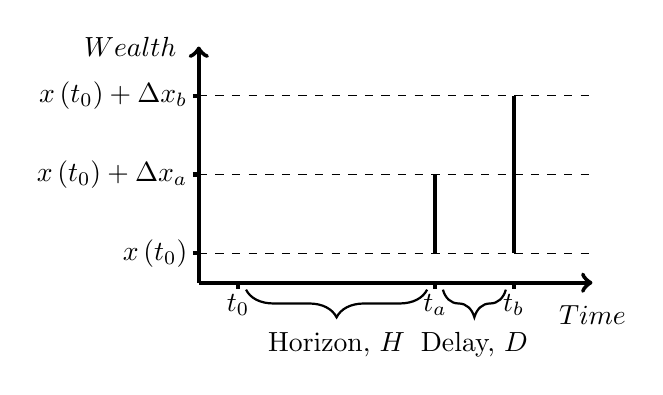
\begin{tikzpicture}[scale=0.50]
%\draw[help lines, color=gray!30, dashed] (-5,0) grid (4.9,5.9);
\draw[->,ultra thick] (-5,0)--(5,0) node[below,yshift=-4pt]{$Time$};
\draw[->,ultra thick] (-5,0)--(-5,6) node[left,xshift=-4pt]{$Wealth$};
\draw[-,ultra thick] (-4,-0.15)--(-4,0) node[below]{$t_0$};
\draw[-,ultra thick] (1,-0.15)--(1,0) node[below]{$t_a$};
\draw[-,ultra thick] (3,-0.15)--(3,0) node[below]{$t_b$};
\draw[-,ultra thick] (-5.15,0.75)--(-5,0.75) node[left]{$x\left(t_0\right)$};
\draw[-,ultra thick] (-5.15,2.75)--(-5,2.75) node[left]{$x\left(t_0\right) + \Dx_a$};
\draw[-,ultra thick] (-5.15,4.75)--(-5,4.75) node[left]{$x\left(t_0\right) + \Dx_b$};
\draw[-, dashed] (-5,0.75)--(5,0.75) ;
\draw[-, dashed] (-5,2.75)--(5,2.75) ;
\draw[-, dashed] (-5,4.75)--(5,4.75) ;
\draw[-, ultra thick] (1,0.75)--(1,2.75) ;
\draw[-, ultra thick] (3,0.75)--(3,4.75) ;
\draw [decorate,decoration={brace,amplitude=10pt,mirror},xshift=0pt,yshift=-5pt,thick](-3.8,0) -- (0.8,0) node [black,midway,yshift=-20pt]{$\text{Horizon, }\hor$};
\draw [decorate,decoration={brace,amplitude=10pt,mirror},xshift=0pt,yshift=-5pt,thick](1.2,0) -- (2.8,0) node [black,midway,yshift=-20pt]{$\text{Delay, }\del$};
\end{tikzpicture}
\caption{The basic setup of the model. A decision maker faces a choice at time $t_0$ between option $a$, which guarantees a payment of $\Dx_a$ at time $t_a$, and option $b$, which guarantees a payment of $\Dx_b>\Dx_a$ at time $t_b>t_a$. We define the time between the decision and the earlier payment as the {\it horizon}, $\hor\equiv t_a-t_0$; and the time between the two payments as the {\it delay}, $\del\equiv t_b-t_a$.}
\flabel{basicsetup}
\end{figure}
\end{frame}

\subsection{What is a growth rate:}
\begin{frame}{What is a growth rate?}

 A growth rate, $g$, is defined as the scale parameter of time for an underlying dynamic of wealth. 

If wealth evolves multiplicatively at rate $r$, it is also the scale parameter, $g=r$(Income generating assets ):

\be
x\left(t\right) = x\left(0\right) e^{r t}\,,
\ee

If additive dynamics, where wealth grows linearly in time at rate $k$, k is the scale parameter(labor income):

\be
x\left(t\right) = k t + x\left(0\right)\,,
\ee

so under multiplicative dynamics: $r = \frac{\log x(t+\Dt)-\log x(t)}{\Dt}$ and under additive dynamics: $k = \frac{x\left(t+\Dt\right)-x\left(t\right)}{\Dt}$.
\end{frame}

\subsection{Axioms and definitions}

\subsubsection{Growth}

\begin{frame}{Growth Axiom}
\begin{definition}{The Maximization of Growth.}
Given the wealth dynamics, a decision time $t_0$, an initial wealth $x\left(t_0\right)$, and payments $a\equiv\left(t_a,\Dx_a\right)$ and $b\equiv\left(t_b,\Dx_b\right)$, such that we have a RIPP:
\begin{itemize}
\item $\left(t_a,\Dx_a\right) \succ \left(t_b,\Dx_b\right)$ if and only if $g_a > g_b$
\item $\left(t_a,\Dx_a\right) \sim \left(t_b,\Dx_b\right)$ if and only if $g_a = g_b$
\item $\left(t_a,\Dx_a\right) \prec \left(t_b,\Dx_b\right)$ if and only if $g_a < g_b$
\end{itemize}
\label{ax:ax1}
\end{definition}
\end{frame}

\subsubsection{Definition of discount rate}
\begin{frame}{Discount rate}
\be
\delta\left(\del\right) \equiv \left.\frac{\Dx_a}{\Dx_b}\right|_{a \sim b}\,.
\ee
\ie the ratio of payoffs under the constraint that the growth rates of wealth are equal.
\end{frame}

\subsection{Model}
\subsubsection{Environment: Adaptive vs Fixed}
\begin{frame}{Environment: Adaptive vs Fixed}
\begin{itemize}
    \item \textbf{Adaptive}: Time of next choice depends on current choice. \textbf{Illustration:} Dana, the real estate developer, loves to work and always wants to keep busy with her building projects, she always gets paid at their completion. Dana has a choice between a project that lasts \textit{three months} and a project that lasts \textit{six months}. 
    \item \textbf{Fixed}: Time of next choice independent on current choice. \textbf{Illustration:} Every january Bob the bureacrat is given a budget. Bob must choose a project to fund with his allocated budget. All projects cost the entire allocated budget(there is no question of saving). He is paid upon the completion of each project.
\end{itemize}
\end{frame}

\subsubsection{Cases}
\begin{frame}{Cases:}
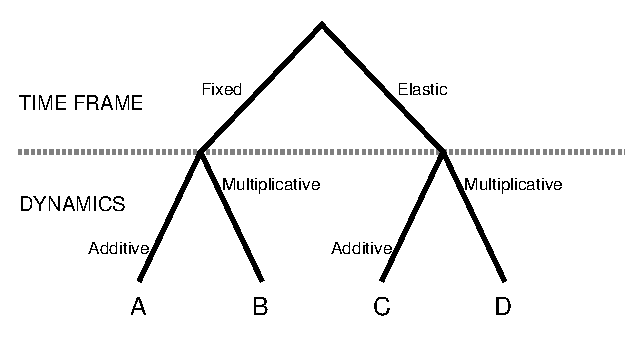
\includegraphics[width=0.7\textwidth]{./figures/tree2.eps} \newline
The four model specifications, determined by specifying a time frame and wealth dynamics. The labels A, B, C, and D, are used for the different cases.
\end{frame}



\subsubsection{A: Fixed time, additive dynamics}
\begin{frame}{A: Fixed time, additive dynamics}
Now we assume additive dynamics as in case A, but with a fixed time frame so that the outcomes of both choices are compared at $t_b$. The wealths evolve to: \bea
x_a\left(t_b\right) &=& x\left(t_0\right) + \Dx_a + k(t_b-t_0)\,; \\
x_b\left(t_b\right) &=& x\left(t_0\right) + \Dx_b + k(t_b-t_0)\,.
\eea
The growth rates are:
\bea
g_a &=& \frac{x_a\left(t_b\right) - x\left(t_0\right)}{t_b-t_0} = \frac{\Dx_a}{t_b-t_0} + k\,;\\
g_b &=& \frac{x_b\left(t_b\right) - x\left(t_0\right)}{t_b-t_0} = \frac{\Dx_b}{t_b-t_0} + k\,.
\eea
Note that the wealth and its growth rate under option $b$ are the same as in case A, since they were already evaluated at $t_b$. Therefore one simply takes the expected value. 
\end{frame}

\subsubsection{B: Fixed time, multiplicative dynamics}
\begin{frame}{B: Fixed time, multiplicative dynamics}
This is the standard case in inter-temporal discounting. Earlier payouts receive interest rate.
\bea
x_a\left(t_b\right) &=& x\left(t_0\right) e^{r(t_b-t_0)} + \Dx_a e^{r(t_b-t_a)}\,;\\
x_b\left(t_b\right) &=& x\left(t_0\right) e^{r(t_b-t_0)} + \Dx_b\,.
\eea
The corresponding growth rates are:
\bea
g_a &=  \frac{1}{t_b-t_0}\log{\left(1 + \frac{\Dx_a e^{r(t_b-t_a)}}{x\left(t_0\right)e^{r(t_b-t_0)}}\right)} +r \\
g_b &=  \frac{1}{t_b-t_0}\log{\left(1 + \frac{\Dx_b}{x\left(t_0\right)e^{r(t_b-t_0)}}\right)} +r \,.
\eea
Note that the evolution of wealth under option $b$ is the same as in case B.
\end{frame}

\begin{frame}{B: Fixed time, multiplicative dynamics(2)}
Thus, $g_a > g_b$ if
\be
\Dx_a e^{r(t_b-t_a)} > \Dx_b\,,
\ee
or, in terms of the delay, if
\be
\Dx_a e^{r\del} > \Dx_b\,.
\ee

The discount factor is similarly expressed by setting the growth rates to be equal. Then we get $\Dx_a e^{r\del} = \Dx_b$ and
\be
\delta = \frac{\Dx_a}{\Dx_b} = e^{-r\del}\,,
\ee
Which is the standard exponential discounting result. Note that, with this specification, the horizon is irrelevant. All that matters is the payoff amount after possible re-investment.
\end{frame}

\subsubsection{C: Adaptive time, additive dynamics}
\begin{frame}{C: Adaptive time frame with additive dynamics}
Dynamics
\bea
x_a\left(t_a\right) &=& x\left(t_0\right) + \Dx_a + k(t_a-t_0)\,;\\
x_b\left(t_b\right) &=& x\left(t_0\right) + \Dx_b + k(t_b-t_0)\,.
\eea
The growth rates are:
\bea
g_a &=& \frac{x_a\left(t_a\right) - x\left(t_0\right)}{t_a-t_0} = \frac{\Dx_a}{t_a-t_0} + k\,;\\
g_b &=& \frac{x_b\left(t_b\right) - x\left(t_0\right)}{t_b-t_0} = \frac{\Dx_b}{t_b-t_0} + k\,.
\eea
It follows that the criterion $g_a > g_b$ is
%
\be
\frac{\Dx_a}{\hor} > \frac{\Dx_b}{\hor +\del}\,.
\elabel{criterion_caseC}
\ee
\end{frame}

\begin{frame}{C: Adaptive time frame with additive dynamics(2)}
Preference reversals are observed changes in decisions as time passes, \ie as the horizon gets shorter. We can test whether they are predicted in our model by varying $\hor$ while holding other variables constant. In the present specification, indifference occurs at the horizon for which \eref{criterion_caseC} becomes an equality, \ie at $\hor=\hor^\text{PR}$ where
\be
\hor^\text{PR} \equiv \frac{\del \Dx_a}{\Dx_b - \Dx_a}\,.
\elabel{HPR}
\ee
It follows that the criterion $g_a = g_b$ gives us the hyperbolic discount rate
\be
\delta = \frac{\Delta a}{\Delta b} = \frac{t_a-t_0}{t_b-t_0}=\frac{1}{1+\frac{D}{H}} \,.
\ee
\end{frame}

\begin{frame}{C: Adaptive time frame with additive dynamics(3)}
We can also determine the exact time, $t_0$, where the change in preferences occurs. 
\be
t_0 = \frac{\Delta x_b t_a - \Delta x_a t_b}{\Delta x_b - \Delta x_a}
\ee
\begin{figure}[!htb]
\centering
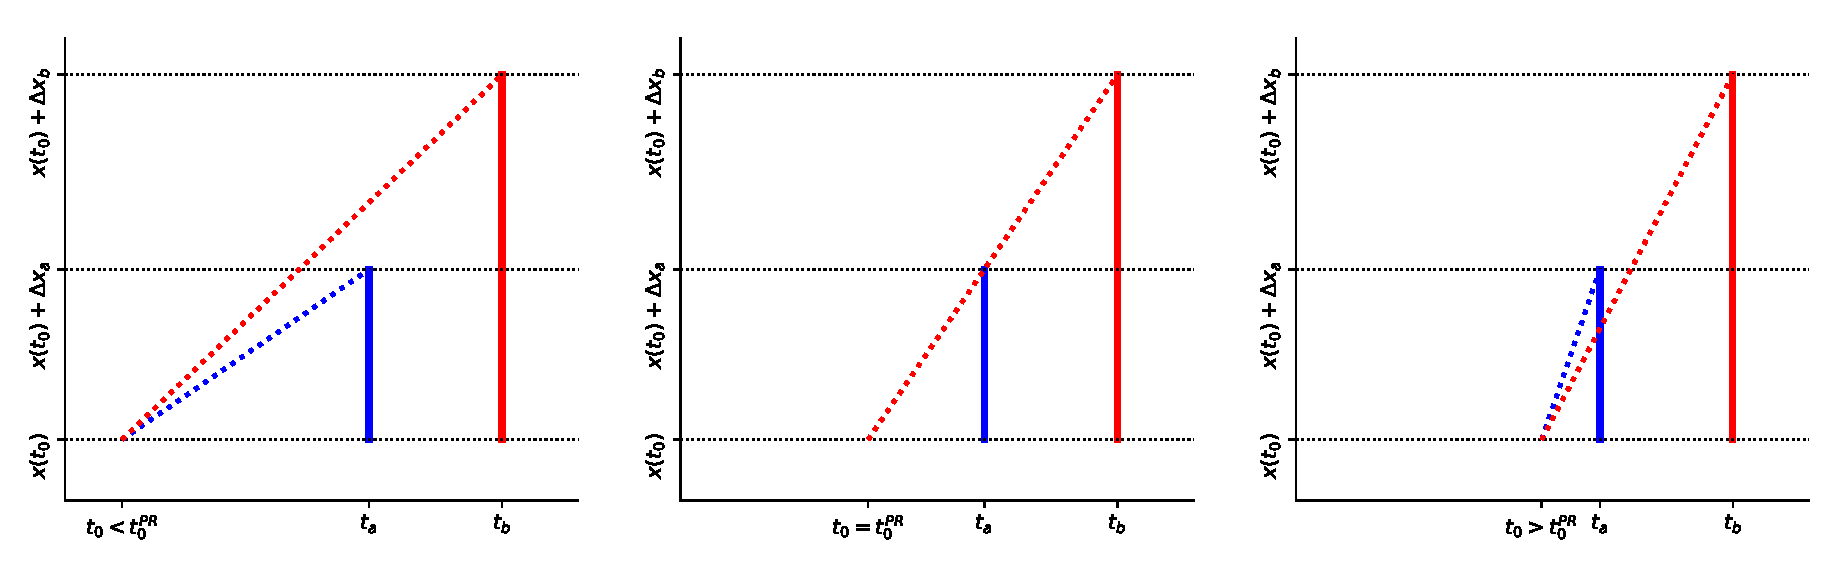
\includegraphics[width=1.0\textwidth]{./figures/reversals.eps}
\caption{Preference reversal in case C. From left to right panel, $t_0$ increases, that is, the time of the payoffs approaches, while all other parameters are unchanged. Initially, option $b$ is preferable, having the higher growth rate.}
\flabel{caseA}
\end{figure}
\end{frame}

\subsubsection{D: Adaptive time, multiplicative dynamics}
\begin{frame}{D: Adaptive time, multiplicative dynamics(1)}
We follow the same steps as in case A. Wealth evolves to:
\bea
x_a\left(t_a\right) &=& x\left(t_0\right) e^{r(t_a-t_0)} + \Dx_a\,;\\
x_b\left(t_b\right) &=& x\left(t_0\right) e^{r(t_b-t_0)} + \Dx_b\,.
\eea

The corresponding growth rates are:
\bea
g_a &=& \frac{\log x_a\left(t_a\right) - \log x\left(t_0\right)}{t_a-t_0} \\&=& \frac{1}{\hor}\log{\left(1 + \frac{\Dx_a}{x\left(t_0\right)e^{r\hor}}\right)} + r \elabel{ga_D}\,;\\
g_b &=& \frac{1}{\hor + \del}\log{\left(1 + \frac{\Dx_b}{x\left(t_0\right)e^{r\left(\hor + \del\right)}}\right)} + r\,.
\elabel{gb_D}
\eea
\end{frame}

\begin{frame}{D: Approximation}
$\delta$ cannot be derived explicitly. However, if we assume small payoffs relative to wealth, \ie $\Dx_a \ll x\left(t_0\right)e^{r(t_a-t_0)}$ and $\Dx_b \ll x\left(t_0\right)e^{r(t_b-t_0)}$, then, setting $g_a=g_b$ and using the first-order approximation $\log(1+\epsilon)\approx\epsilon$ for $\epsilon\ll1$, we get
\be
\Dx_b > \Dx_a e^{r\del}\left(\frac{\hor+\del}{\hor}\right)\,,
\ee
\end{frame}




\begin{frame}{D: Delta in the small payment limit}

\be
\delta\left(\del;\hor;r\right) = \left.\frac{\Dx_a}{\Dx_b}\right|_{g_a=g_b} \approx \frac{\hor e^{r\hor}}{\left(\hor + \del\right)e^{r\left(\hor + \del\right)}} = \frac{e^{-r\del}}{1+\del/\hor}\,
\ee
the interest rate remains
\end{frame}


\begin{frame}{D: Numerical Example:}
Suppose an agent faces a choice between receiving $\$10$ after 1 year (choice a) or $\$25$ after two years (choice b), and we assume the agent has no access to a rate of interest. The model states that the agent will evaluate the following for a and b:

\be
g_a = \frac{1}{1}\log\left(\frac{100 + 10}{100}\right) \approx 0.095\text{~per annum}\,.
\ee

\be
g_b = \frac{1}{2}\log\left(\frac{100 + 25}{100}\right) \approx 0.112\text{~per annum}\,.
\ee

Therefore, the agent would prefer the later option because $0.112 > 0.095$. Now suppose that the agent has initially only $\$10$, a similar calculation yields $g_a\approx0.69$ and $g_b\approx0.63$. This means that a poorer individual would prefer the earlier choice.
\end{frame}

\begin{frame}{D: Wealth effect}
\begin{figure}[!htb]
\centering
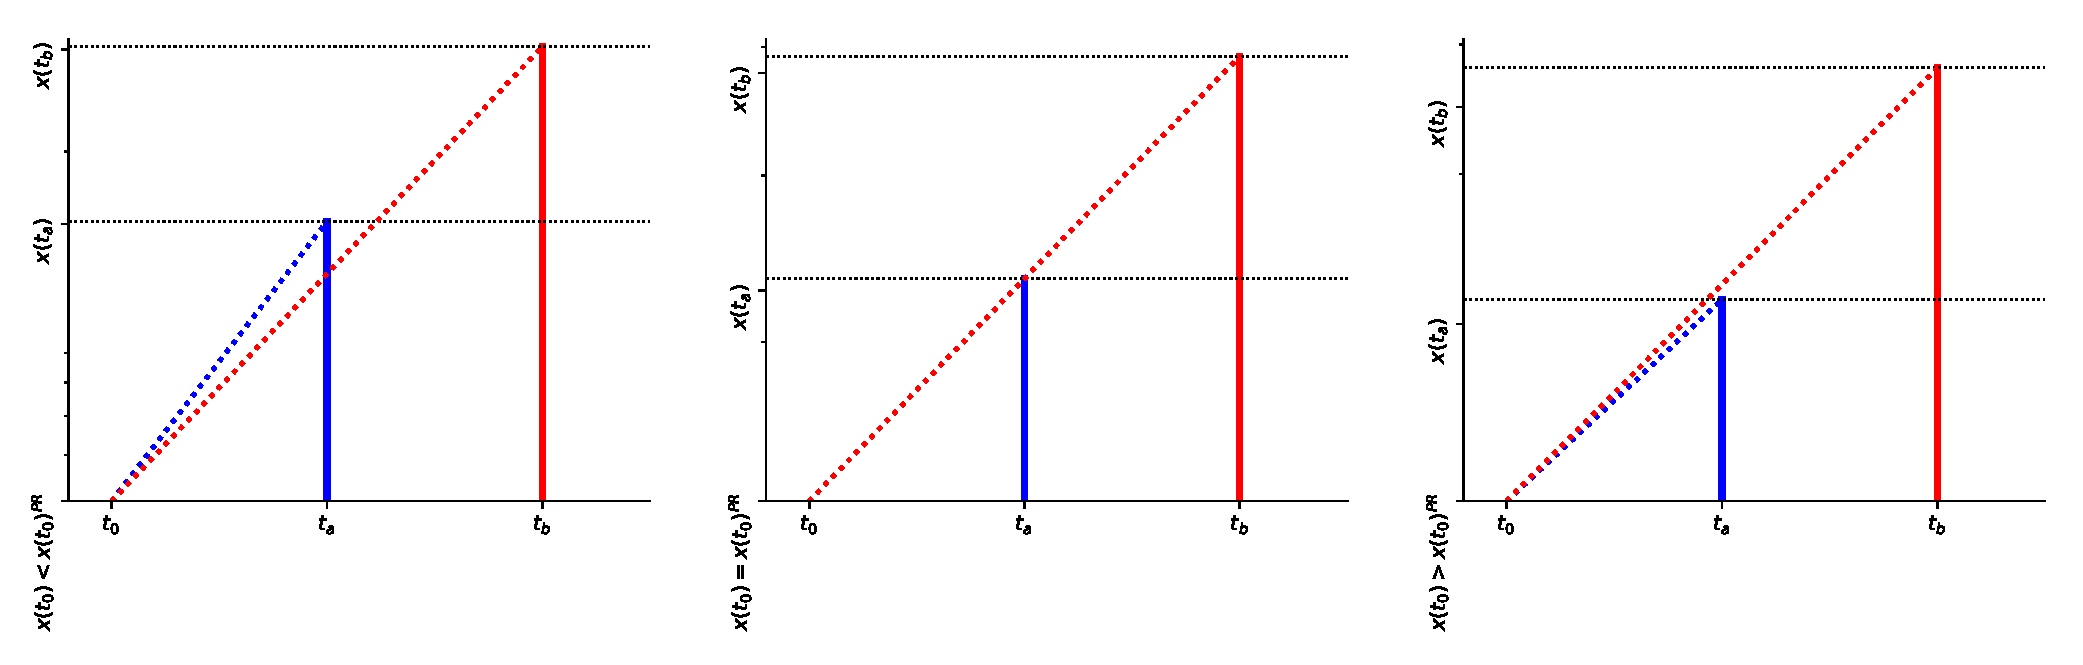
\includegraphics[width=1.0\textwidth]{./figures/reversals_B.eps}
\caption{Initial wealth $x(t_0)$ increases from left to right panel (\$500, \$2277, \$5,000), while all other parameters are unchanged ($t_0=$ today, $t_a=1$~year from today, $t_b=2$~years from today, $\Dx_a=\$1000$, $\Dx_b=\$2500$, $r=0.03$~per annum). 
$x(t_0)^{PR}\approx \$2277$, both options imply equal growth}
\flabel{reversal_B}
\end{figure}
\end{frame}

\begin{frame}{D: Simulation of the wealth effect}
The difference $g_a-g_b$, is shown as a function of $x(t_0)$ in~\fref{reversal_B2}. 

\begin{figure}[!htb]
\centering
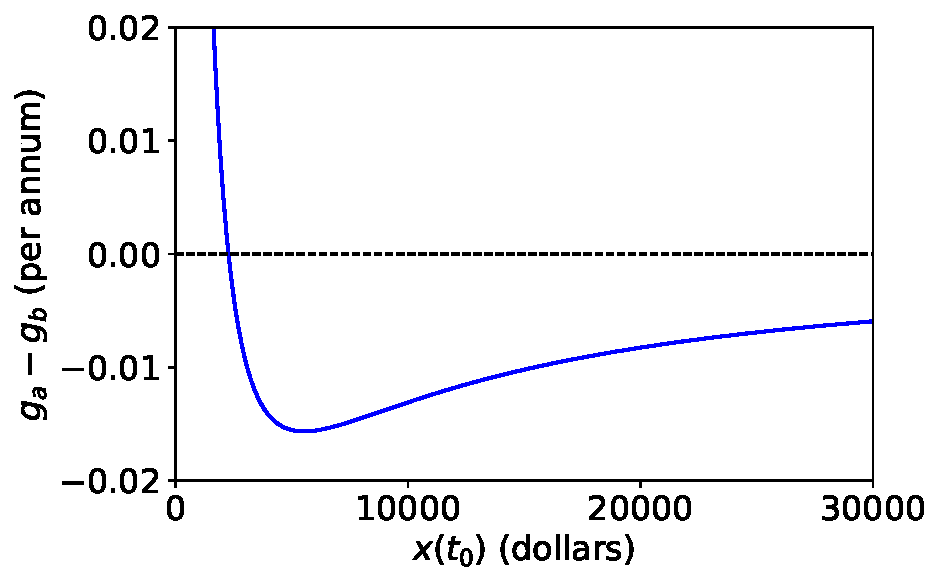
\includegraphics[width=0.7\textwidth]{./figures/ga_gb.pdf}
\caption{The difference $g_a-g_b$ is positive when the earlier payoff is preferable, and otherwise negative. We see that for small initial wealths $x(t_0)$ the earlier smaller payoff is preferred, whereas for large initial wealth the later larger payoff is preferred (parameters as in~\fref{reversal_B}).}
\flabel{reversal_B2}
\end{figure}
\end{frame}

\subsection{Comparison and conclusion}
\begin{frame}{Comparison}
\begin{figure}[!htb]
\centering
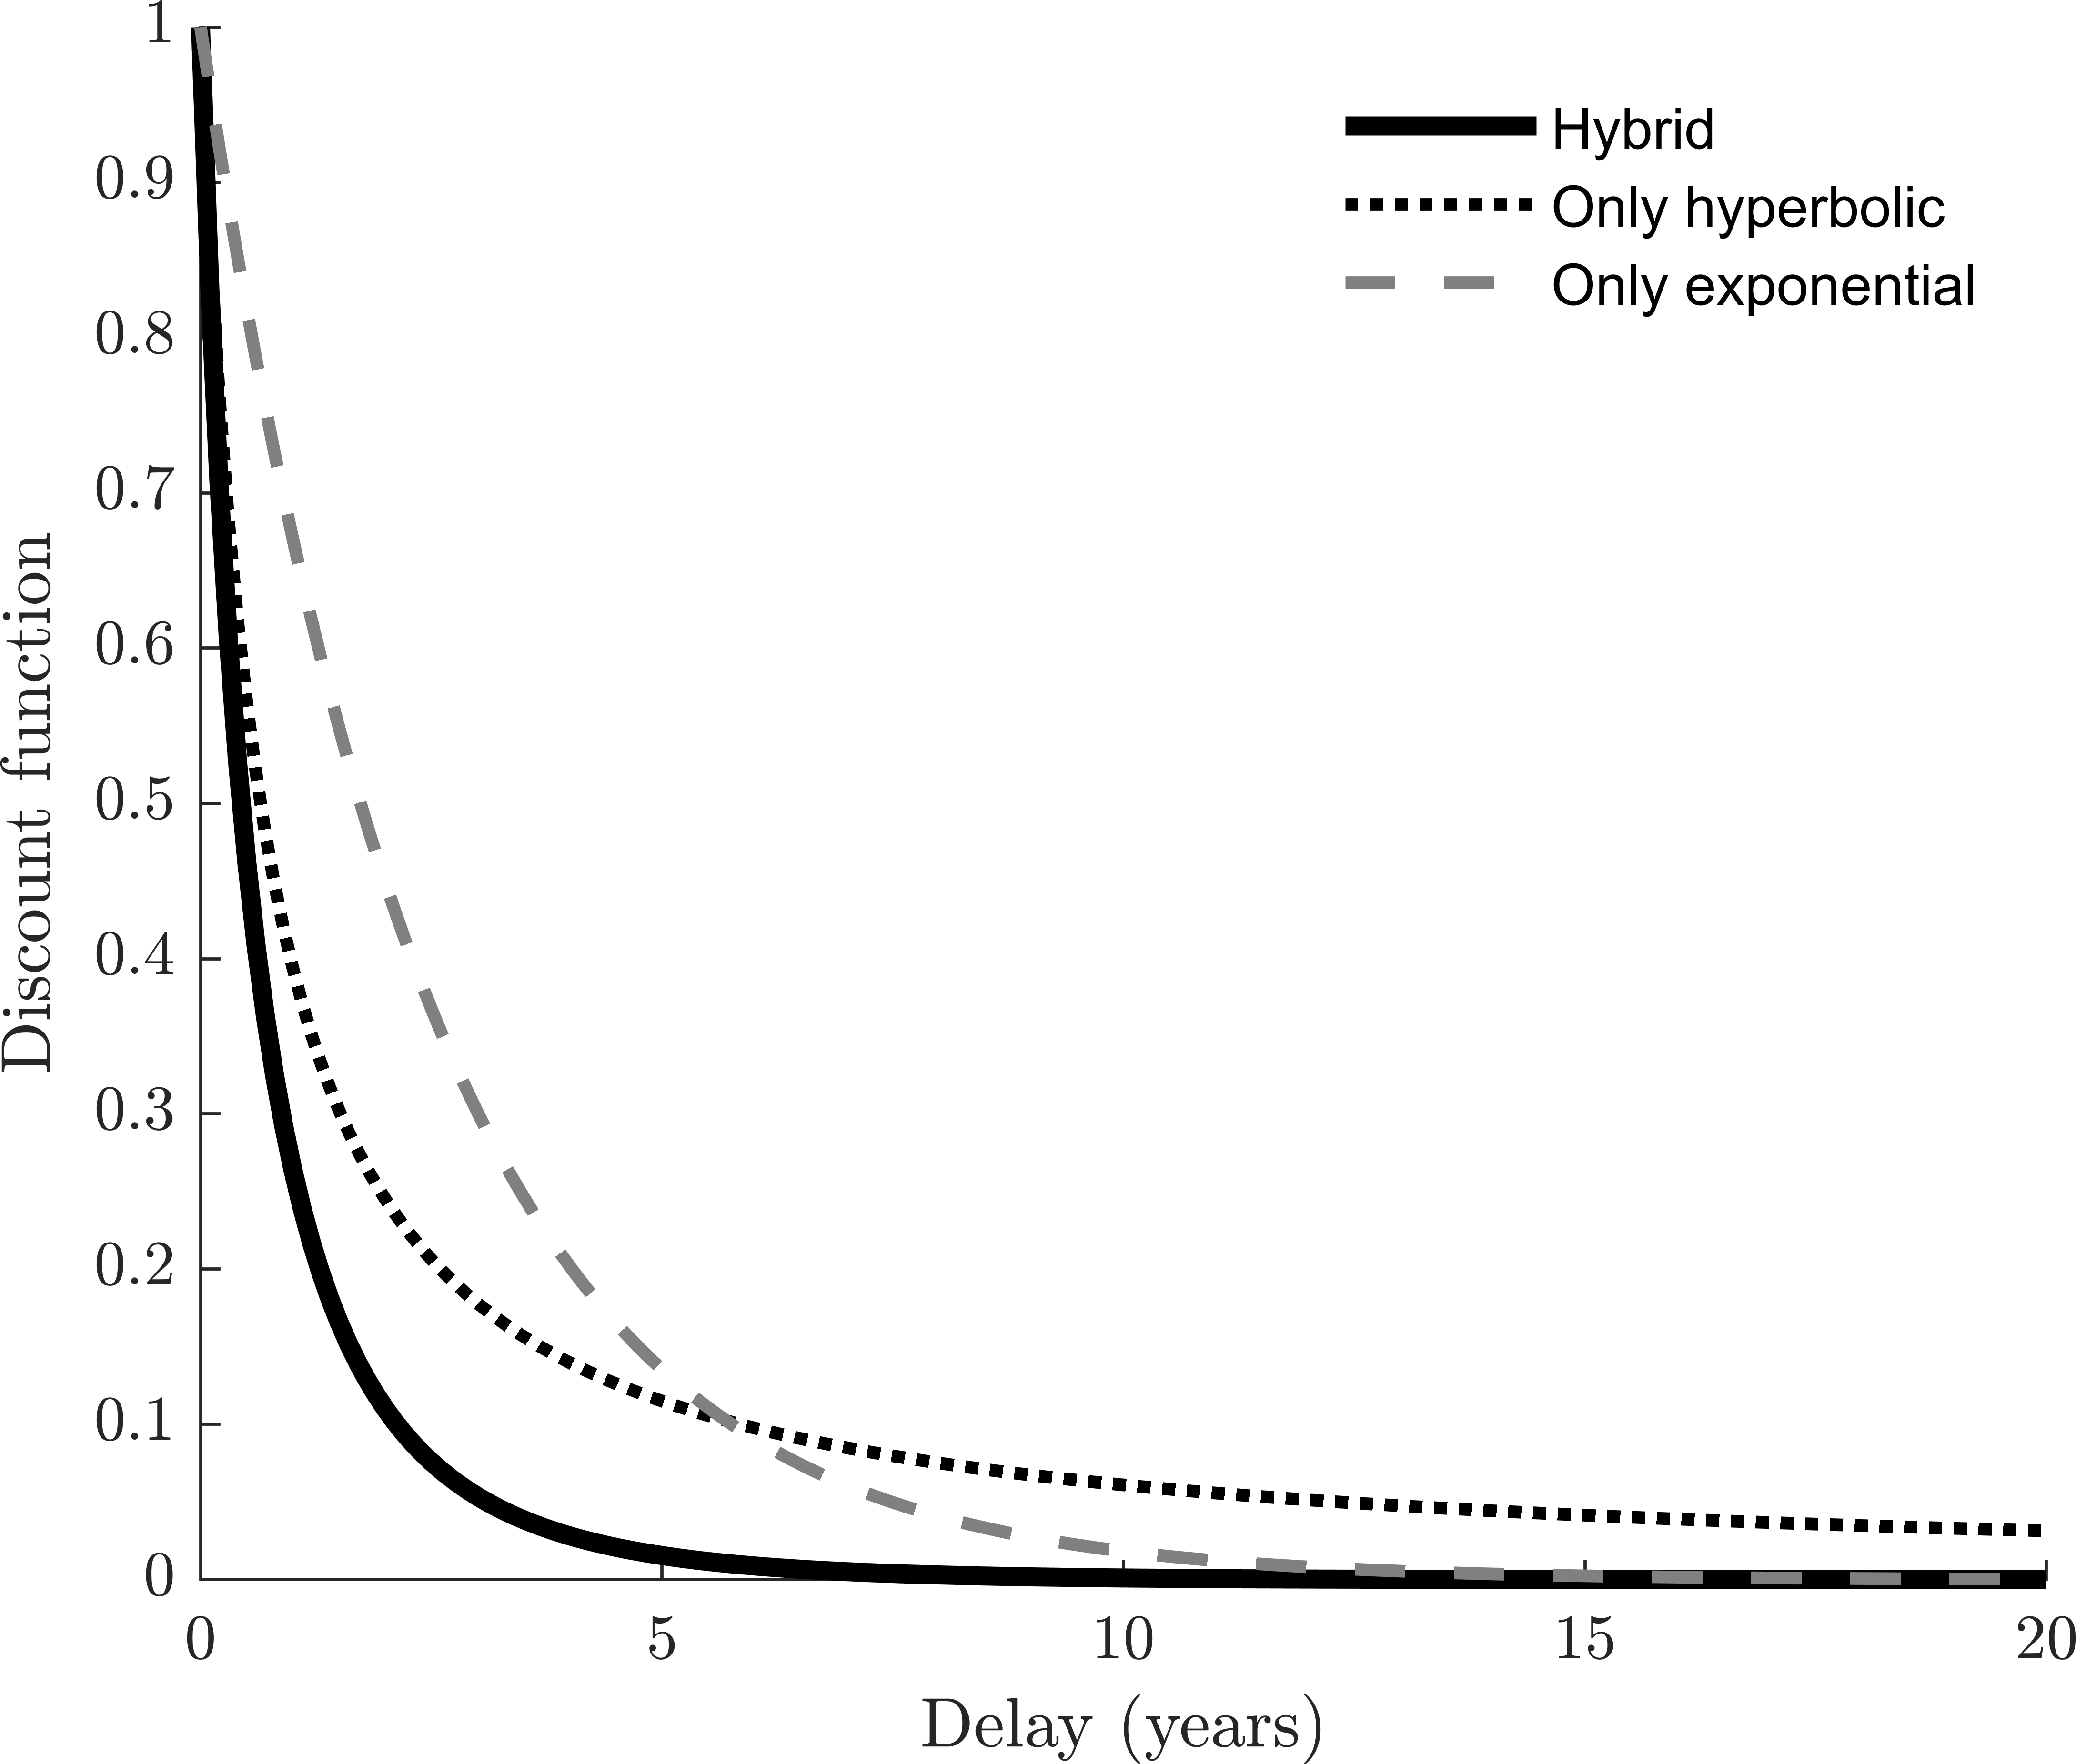
\includegraphics[width=0.7\textwidth]{./figures/caseD_delta_asymptotic2.jpg}
\caption{The discount function in the small payment limit in case D. The solid black curve is the hybrid $\delta = e^{-r\del}/(1+\del/\hor)$, for $r=0.4\text{ per annum}$ and $\hor=0.65\text{ years}$. This is close to the hyperbolic discount function $1/(1+\del/\hor)$ (black dotted) for short delays and to the exponential discount function $e^{-r\del}$ (grey dashed) for long delays.}
\flabel{shortpaymentasymp}
\end{figure}
\end{frame}



\begin{frame}{Empirical Implication}
\begin{itemize}
    \item Wealthy vs non-wealthy: \citep{GreenETAL1996,EpperETAL2018}
    \item \textbf{Predictions:}
    \item Among rich people, hyperbolic for short delays, exponential for long delays
    \item A single crossing preference reversal
    \item People whose future choices depend on current choices will behave more hyperbolically. (Entrepreneurs) 
    \item If there is a limited use of an item/skill/action per period, agents will discount less
    \item Income generating assets owners will discount the most
\end{itemize}
\end{frame}



\begin{frame}{Conclusive comments }
\begin{itemize}
    \item We show that expected value, exponential, hyperbolic and payoff per unit of time are all special cases of the environment.
    \item We show that discounting can be objective (does not depend on preferences)
    \item We introduce a new concept having to do with the adaptiveness of the action set to time
\end{itemize}
\end{frame}

\begin{frame}
\bibliographystyle{aea}
\small{
\bibliography{../LML_bibliography/bibliography}}
\end{frame}

\end{document}